\documentclass[letterpaper,12pt]{article}
\usepackage{tabularx} % extra features for tabular environment
\usepackage{amsmath}  % improve math presentation
\usepackage{graphicx} % takes care of graphic including machinery
\usepackage[margin=1in,letterpaper]{geometry} % decreases margins
\usepackage{cite} % takes care of citations
\usepackage[final]{hyperref} % adds hyper links inside the generated pdf file
\hypersetup{
	colorlinks=true,       % false: boxed links; true: colored links
	linkcolor=blue,        % color of internal links
	citecolor=blue,        % color of links to bibliography
	filecolor=magenta,     % color of file links
	urlcolor=blue         
}
\usepackage{blindtext}
\usepackage{mathtools}
\usepackage{tikzsymbols}

\DeclarePairedDelimiter\ceil{\lceil}{\rceil}
\DeclarePairedDelimiter\floor{\lfloor}{\rfloor}
%++++++++++++++++++++++++++++++++++++++++


\begin{document}

\title{Proyecto 2 --- Sudoku Solver Mejorado}
\author{David Segura 13-11341 \& Amin Arriaga 16-10072}
\date{17 de Julio, 2020}
\maketitle

\begin{abstract}
En este proyecto aplicamos todo el contenido estudiado en la materia Diseño de Algoritmos I dictada por el profesor Ricardo Monascal. \textbf{Nota especial:} Gran reconocimiento de agradecimiento al estudiante Amin Arriaga por decidirse a cursar la materia (by D10S).
\end{abstract}


\section{Introducción}

Esta implementación es una continuación del anterior proyecto. Esta etapa consiste en la mejoría del tiempo de ejecución en el resolvedor de \textbf{SAT} mediante estrategias que explicaremos posteriormente.

\section{Mejoras de SAT}

\subsection{Idea presentada en el Proyecto}

La propagación unitaria propuesta por los profesores del curso en el enunciado del proyecto, es un concepto que ya estábamos aplicando en nuestra implementación para la primera parte. Sin embargo, se desarrollaron dos nuevas estructuras para la optimización de la ejecución: \texttt{Variable}, \texttt{Closure} y \texttt{CNF}.

\begin{itemize}
	\item \texttt{Variable:} Se implementó esta clase para tener una estructura de datos que almacene los datos correspondiente a una variable, los cuales son: las clausulas en las que la variable aparece, el signo que tiene asignado y un \textit{backup} donde se guardan el signo del literal en distintos estados de ejecución.
	
	Los métodos que esta clase tiene son:
	\begin{itemize}
		\item \texttt{\_\_init\_\_}: Inicializa la instancia con \texttt{sign = 0}, \texttt{closures = []} y \texttt{backup = \{\}}
		
		\item \texttt{assign}: Se encarga de asignarle el signo al literal.
		
		\item \texttt{add\_closure}: Agrega una clausula a la información del literal.
	    
	    \item \texttt{save}: Guarda una copia del signo actual.
	    
	    \texttt{restaure}: Método que restablecerá una copia guardada mediante la llave indicada, eliminando dicha informaci\'on del backup para no acumularla. Se utiliz\'o un diccionario y no una pila de eventos pues, por alguna raz\'on, con la pila no se almacenaban/restauraban los datos en el orden correcto, mientras con la llave, podemos estar seguros de que el estado a restaurar ser\'a el correcto.
	\end{itemize}
	
	Todos los m\'etodos tienen complejidad en tiempo y memoria de $O(1)$.

	\item \texttt{Closure:} Se implementó esta clase para tener una estructura de datos que almacene los datos correspondiente a una clausula, los cuales son: los literales que pertenecen a la misma, el tamaño de la clausula, una variable que indica si fue satisfecha (si ya tomó valor de \textit{True} mediante alguno de sus literales), y un \textit{backup} donde se guardan toda esta informaci\'on ya mencionada en distintos estados de ejecución.
	
	Los métodos que esta clase tiene son:
	\begin{itemize}
		\item \texttt{\_\_init\_\_}: Inicializa la instancia con \texttt{literales = []}, \texttt{N = 0}, \texttt{satisfied = False} y \texttt{backup = \{\}}.
		
		\item \texttt{add}: Agrega un literal a la clausula.
		
		\item \texttt{delete}: Se encarga de eliminar los literales indicados pertenecientes a la clausula. Devuelve un booleano que indica si la clausula quedó vacía o no.
	    
	    \item \texttt{save}: Guarda una copia de toda la información almacenada en la clausula.
	    
	    \texttt{restaure}: Restablecerá una copia guardada mediante la llave indicada, eliminando dicha informaci\'on del backup para no acumularla. Se uso un diccionario y no una pila de eventos por las mismas razones indicadas en la descripci\'on de la clase \texttt{Variable}.
	\end{itemize}
	
	\textbf{Tiempo Asintóstico:}
    \begin{itemize}
    	\item \texttt{\_\_init\_\_}, \texttt{add}, \texttt{save}, \texttt{restaure} $\in O(1)$.
    	
    	\item \texttt{delete} $\in O(d)$, siendo $d$ la cantidad de elementos a eliminar.
    \end{itemize} 
    
    \textbf{Memoria Asintótica:}
    \begin{itemize}
    	\item \texttt{add}, \texttt{delete}, \texttt{restaure} $\in O(1)$.
    	\item \texttt{save} $\in O(l)$, siendo $l$ el n\'umero original de literales en la cl\'ausula.
    \end{itemize}
    
    \item \texttt{CNF:} Se implement\'o esta clase para almacenar todas las cl\'ausulas del problema y el n\'umero de cl\'ausulas que quedan sin satisfacer. El principal objetivo de esta clase es no tener que verificar cada cl\'ausula para decidir si el problema ya fue resuelto o no. Al igual que las clases anteriores, contiene un backup, pero almacena \'unicamente el n\'umero de cl\'ausulas que ten\'ia en ese momento.
    
    Los métodos que esta clase tiene son:
	\begin{itemize}	   
		\item \text{\_\_init\_\_}: Inicializa la instancia con \texttt{closures = closures}, \texttt{N = 0} y \texttt{backup = \{\}}, siendo \textit{closures} una lista de lista de cl\'ausulas, donde si una cl\'ausula se encuentra en la $i$-\'esima lista, significa que tiene $i+1$ literales. A esta lista de lista de cl\'asusulas la denominaremos \texttt{C} el resto del informe.
		 
	    \item \texttt{save}: Guarda una copia del n\'umero de cl\'ausulas en ese momento.
	    
	    \texttt{restaure}: Restablecerá una copia guardada mediante la llave indicada, eliminando dicha informaci\'on del backup para no acumularla. Se uso un diccionario y no una pila de eventos por las mismas razones indicadas en la descripci\'on de la clase \texttt{Variable}.
	\end{itemize}
	
	Todos los m\'etodos tienen complejidad en tiempo y memoria de $O(1)$. Podr\'ia parecer que \texttt{\_\_init\_\_} $\in O(|C|)$, sin embargo, solo se guarda una referencia a dicho arreglo, no una copia.
\end{itemize}

Cabe destacar que en nuestra implementaci\'on se usar\'a la misma llave (key) para el backup de las variables, de \texttt{C} y de la instancia de \texttt{CNF} en un estado determinado del problema.



\subsection{SAT Solver}

Las funciones usadas por nuestro SAT solver original fueron modificadas para mejorar la eficiencia en la ejecución \texttt{laura\_SAT}:\\

\begin{itemize}
	\item \texttt{update\_C}: A diferencia de antes donde teniamos que buscar en los literales de todas las cl\'ausulas alguna instancia de la variable especificada, ahora simplemente revisamos las cl\'ausulas a las que la variable apunta, por lo tanto nos ahorramos dicha b\'usqueda. Al principio se verifica si la cl\'ausula es satisfecha, en caso de ser asi se pasa a la siguiente cl\'ausulas. Esta verificaci\'on es necesaria pues los apuntadores de las variables hacia las distintas cl\'ausulas donde aparecen nunca son modificados, incluso si la cl\'ausula es satisfecha. Esto nos ayuda a no tener que realizar un backup de todas las referencias a las cl\'ausulas pues estas son invariantes.\\
	
	Luego, se revisan los literales de cada cl\'ausula hasta que no quede ninguno o hasta que alguno de \texttt{True}. Si ocurre el primer caso, todos los literales falsos ser\'an eliminados de la cl\'ausula y se actualizar\'a su posici\'on en \texttt{C}. Si la cl\'ausula queda vac\'ia, significa que dio \texttt{False}, y por lo tanto se retorna \texttt{True} indicando un conflicto. Mientras que para el segundo caso, se elimina la referencia a la cl\'ausula en \texttt{C} y se coloca como satisfecha. Si ninguna cl\'ausula da conflicto, se retorna \texttt{False}.
	
	\item \texttt{verify\_units}: Gracias a \texttt{C}, la estructura de esta funci\'on es mucho m\'as simple, pues simplemente tenemos que verificar \texttt{C[0]} para saber si hay cl\'ausulas unitarias, en vez de buscar entre todas las cl\'ausulas. As\'i, mientras \texttt{|C[0]|>0}, significa que a\'un quedan cl\'ausulas unitarias, se toma una, se coloca como satisfecha y se le asigna True a su literal. Luego, se llama a la funci\'on \texttt{update\_C} para actualizar las cl\'ausulas afectadas.
	
	\item \texttt{search\_amin\_zero}: Funciona exactamente igual que antes, s\'olo que ahora funciona con arreglos de instancia de la clase \texttt{Variable} y no de enteros.
	
	\item Se crea el procedimiento \texttt{restaure} que, dada una llave, restaura el estado de las variables, de \texttt{C} y de la instancia de \texttt{CNF} al momento en que se les realiz\'o un backup usando dicha llave.
	
	\item \texttt{laura\_SAT}: Ahora la verificaci\'on de cl\'ausulas unitarias se realiza justo al principio de la funci\'on. En caso de que no de conflicto y el problema a\'un no est\'e resuelto, se elegir\'a una llave tal que no est\'e siendo usada en el backup de la primera variable, recordemos que todas las instancias a las distintas clases comparten las mismas llaves. Luego, se guardar\'a el estado actual de las variables y las cl\'ausulas. El resto de la funci\'on es practicamente igual, con la diferencia de que se restauran los valores de las variables y las cl\'ausulas cuando ocurre un conflicto con la asignaci\'on \texttt{True} de la variable por el bactracking. No se restaura el estado con la asignaci\'on \texttt{False} pues en caso de dar conflicto, la funci\'on retorna un valor; si la funci\'on es la llamada originalmente significa que no hay soluci\'on, as\'i que no vale la pena restaurar el estado, y si es una llamada recursiva, el estado ser\'a restaurado en la llamada anterior.
\end{itemize}

\textbf{Tiempo Asintóstico:}

\begin{itemize}
	\item \texttt{update\_C} $\in O(|C|*l_{max})$, siendo $|C|, l_{max}$ el n\'umero de cl\'ausulas y el m\'aximo entre el n\'umero de literales de las cl\'ausulas respectivamente.
	
	\item \texttt{verify\_units} $\in O(|V|*O($\texttt{update\_C}$)) = O(|V|*|C|*l_{max})$. Esto se debe a que \texttt{verify\_units} llama a \texttt{update\_C} por cada cl\'ausula unitaria, sin embargo, no puede encontrar m\'as de $|V|$ cl\'ausulas unitaria sin obtener un conflicto, pues significa que se realizaron m\'as de $|V|$ asignaciones a las $|V|$ variables.
	
	\item \texttt{search\_amin\_zero} $\in O(|V|)$ siendo $|V|$ el n\'umero de variables.
	
	\item \texttt{restaure} $\in O(|V| + |C|)$. 

	\item \texttt{laura\_SAT}: Siguiendo la misma l\'ogica al calcular la complejidad de \texttt{laura\_SAT} en el proyecto 1, una cota superior es obviamente $O(2^{|V|})$, sin embargo, para el caso promedio del sudoku, toda la complejidad recaer\'a en \texttt{verify\_units}, que en ese caso ser\'ia $O(|V|*|C|*l_{max})$.
\end{itemize}

\textbf{Memoria Asintótica:} 
\begin{itemize}
	\item \texttt{update\_C} $\in O(l_{max})$.

	\item \texttt{verify\_units} $\in O(1)$.
	
	\item \texttt{search\_amin\_zero} $\in O(1)$.
	
	\item \texttt{restaure} $\in O(1)$.

	\item \texttt{laura\_SAT}: El peor caso ocurre cuando todas las variables son asignadas por decisi\'on del backtraking y no de \texttt{verify\_units}, pues se har\'ia un backup del estado actual en cada asignaci\'on. Luego, en cada asignaci\'on se usa memoria  $O(|V| + |C|*l_{max})$. Por lo tanto, como hay $|V|$ variables, entonces la memoria asint\'otica es $O(|V|^2 + |V|*|C|*l_{max})$.
\end{itemize}

\section{Conclusiones}

Para concluir, realizamos la comparativa de nuestra implementacio\'on actual de \texttt{laura\_SAT} con la anterior, el cual dio una mejora bastante considerable. Los resultados que obtuvimos en este proyecto y en el anterior fueron los siguientes:

	\begin{center}
		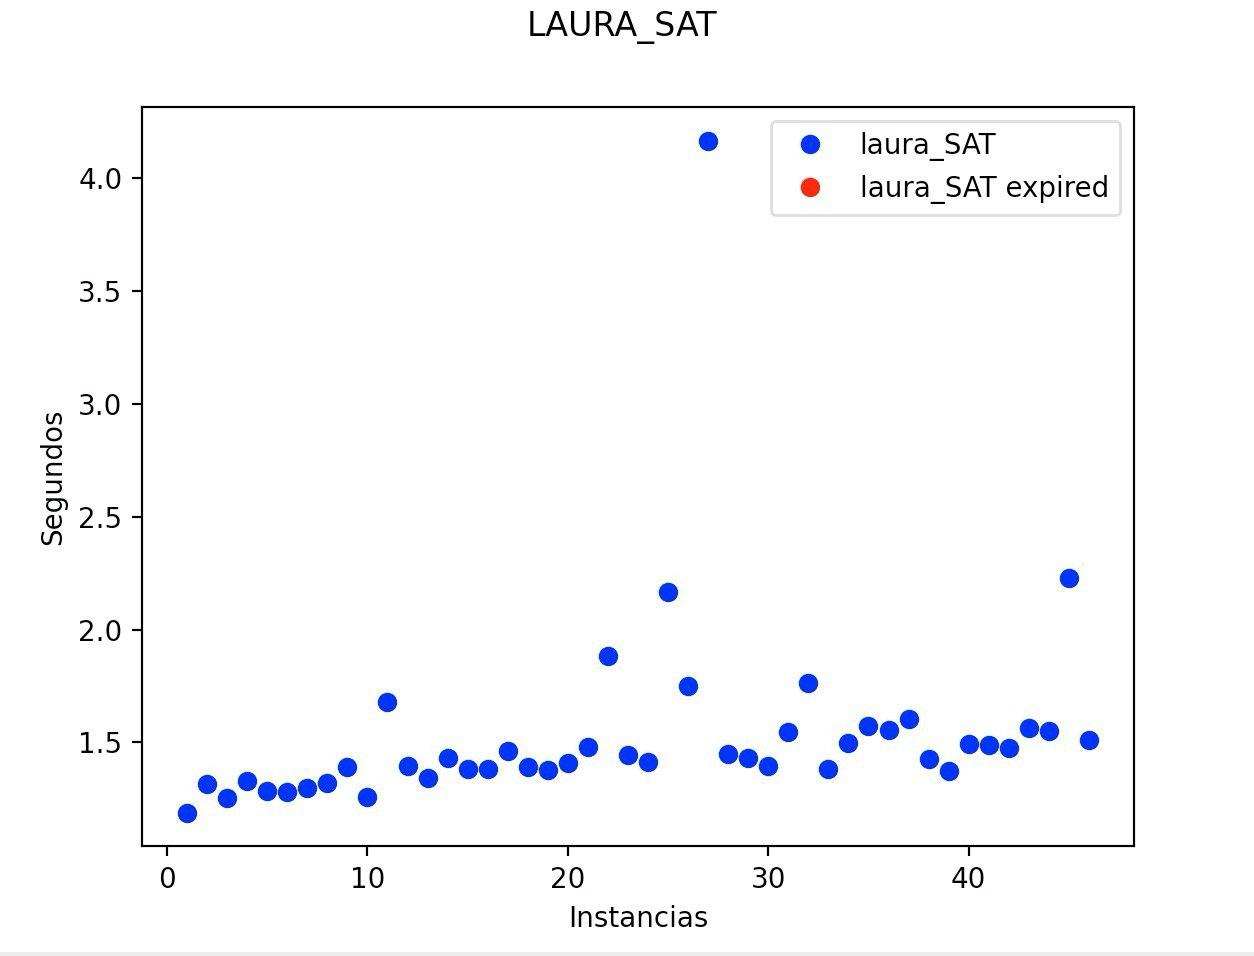
\includegraphics[scale=0.17]{Grafica1.jpg}
		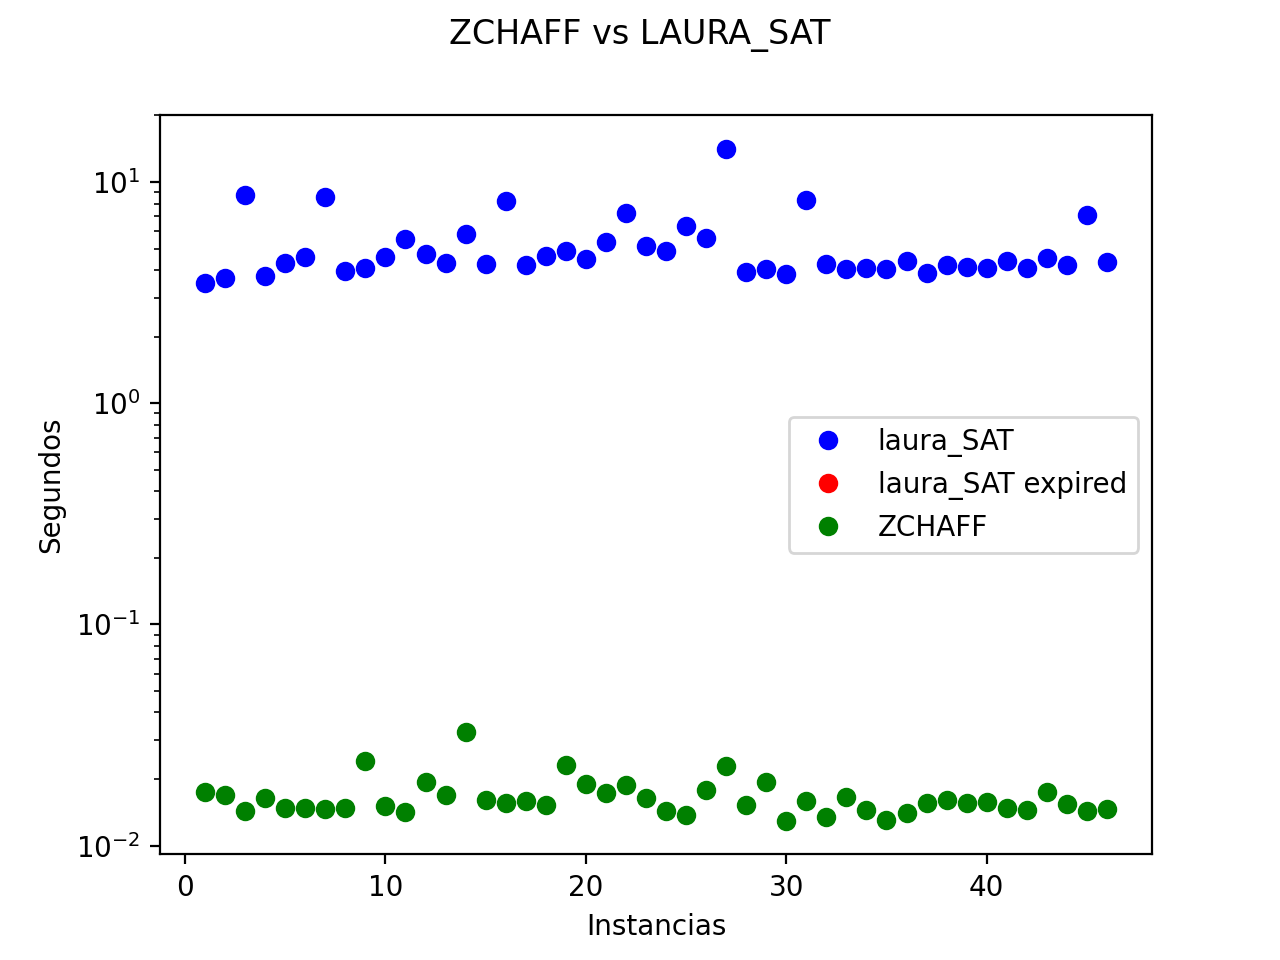
\includegraphics[scale=0.48]{Grafica2}
	\end{center}
	
Donde el peor tiempo fue de poco m\'as de 4 segundos y el promedio 1.5 segundos, a diferencia del proyecto anterior en el que el peor caso fue de alrededor de 11 segundos y el promedio fue de 4 segundos, lo que supone una ejecuci\'on 3 veces m\'as r\'apida aproximadamente. Esto se debe a que se evitaron muchas b\'usquedas entre las cl\'ausulas, ya sea para verificar si todas est\'an vac\'ias, buscar las unitarias o las instancias de las variables, y todo gracias a los apuntadores que hay entre cl\'ausulas y variables.

\end{document}
